\pdfminorversion=7%
\documentclass[aspectratio=169,mathserif,notheorems]{beamer}%
%
\xdef\bookbaseDir{../../bookbase}%
\xdef\sharedDir{../../shared}%
\RequirePackage{\bookbaseDir/styles/slides}%
\RequirePackage{\sharedDir/styles/styles}%
%
\title{Comparing Optimization Algorithms}%
%
\begin{document}%
\startPresentation%
%
\section{Introduction}%
%
\begin{frame}%
\frametitle{Introduction}%
\begin{itemize}%
\item There are many optimization algorithms.%
\item<2-> For solving an optimization problem, we want to use the algorithm most suitable for it.%
\item<3-> \alert<3>{What does this mean?}%
\item<4-> \alert<4>{And how do we find this algorithm?}%
\item<5-> Hopefully this lesson will help answering these questions.%
\item<6-> As a complement to this lesson, I suggest the report \emph{\citetitle{BBDvdBBCEFKLCLIMMNOVWW2020BIOBPAOI}}\cite{BBDvdBBCEFKLCLIMMNOVWW2020BIOBPAOI} on arXiv.%
\end{itemize}%
\end{frame}%
%
%
\begin{frame}[t]%
\frametitle{Exact vs.\ Heuristic Algorithms}%
\begin{itemize}%
\item In optimization, there exist \alert{exact} and \alert{heuristic} algorithms.%
%
\item<2-> Let's look at the classical \glsFull{optTSP}\cite{ABCC2006TTSPACS,LLRKS1985TTSPAGTOCO,GP2002TTSPAIV,WCLTTCMY2014BOAAOSFFTTSP,LWLvdBTW2024ATTSPWFFAAHA,WWCTL2016GVLSTIOPSOEAP}.%
\only<6>{\item<6-> What does \alert{exponential growth} mean?}%
\only<6-7>{\item<6-> Let's say we have a number of cities~$s$\only<-6>{.}\uncover<7->{ and a runtime as a function~$f(s)$ in this log-log plot.}}%
\only<8>{\item<8-> A linear function means that the runtime~$f(s)$ grows slowly with~$s$.}%
\only<9>{\item<9-> A quadratic function (a straight line in log-log plots) is also OK.}%
\only<10-11>{\item<10-> A quartic function \only<-10>{$f(s)=s^4$ gets quite large for growing~$s$}\only<11>{exceeds the number of milliseconds per day at~$s\approx512$}.}%
\only<12-13>{\item<12-> \only<-12>{But this is nothing compared to the exponential function~$f(s)=1.1^s$\dots}\only<13->{A runtime of~$1.1^s$ becomes infeasible for~$s>512$.}}%
\only<14-15>{\item<14-> For larger bases, the runtime grows even faster.}%
\only<16>{\item<16-> If we would enumerate all possible tours of $s$~cities in a \gls{optTSP}, that would be~\factorial{s}.}%
\only<3-5,17->{%
\begin{itemize}%
\only<-5>{\item Clearly, there is (at least) one shortest tour.}%
\only<-8>{\item<5-> \only<-5>{Theory proofs that the time needed to find this tour may grow exponentially with the number~$s$ of cities we want to visit in the worst case.\cite{LLRKS1993SASAAC,CPW1998AROMSCAAA,C1971TCOTPP,K1972RACP,A2008TLOQC}}%
\only<17->{\item Finding the best tour (what exact algorithms do) may take too long.}}%
\only<-19>{\item<18-> But we can find just \alert{some} tour very quickly.}%
\only<-20>{\item<19-> Of course the quality of that tour will be lower\only<20>{: the tour will be longer than the best one}.}%
\only<-22>{\item<21-> Is there something in between?}%
\only<-23>{\item<22-> (Meta-)Heuristic optimization algorithms try to find solutions which are as good as possible as fast as possible.}%
\item<23-> \alert{Optimization often means to make a trade-off between solution quality and runtime.}%
\end{itemize}%
}%
\end{itemize}%
%
\strut\\\strut\\\strut\\\strut\\\strut\\\strut\\\strut\\\strut\\\strut\\\strut\\\strut\\\strut\\\strut\\\strut\\\strut\\\strut\\\strut\\\strut\\\strut%
%
%
\locateGraphic{2-3}{width=0.5\paperwidth}{\sharedDir/graphics/tsp_china/tsp_china_solution}{0.25}{0.29}%
\locateGraphic{4-5}{width=0.58\paperwidth}{\sharedDir/graphics/runtime_quality_tradeoff/runtime_quality_tradeoff_1}{0.21}{0.38}%
%
\locateGraphic{6}{width=0.8\paperwidth}{\sharedDir/graphics/function_growth/function_growth_01}{0.1}{0.29}%
\locateGraphic{7}{width=0.8\paperwidth}{\sharedDir/graphics/function_growth/function_growth_02}{0.1}{0.29}%
\locateGraphic{8}{width=0.8\paperwidth}{\sharedDir/graphics/function_growth/function_growth_03}{0.1}{0.29}%
\locateGraphic{9}{width=0.8\paperwidth}{\sharedDir/graphics/function_growth/function_growth_04}{0.1}{0.29}%
\locateGraphic{10}{width=0.8\paperwidth}{\sharedDir/graphics/function_growth/function_growth_05}{0.1}{0.29}%
\locateGraphic{11}{width=0.8\paperwidth}{\sharedDir/graphics/function_growth/function_growth_06}{0.1}{0.29}%
\locateGraphic{12}{width=0.8\paperwidth}{\sharedDir/graphics/function_growth/function_growth_07}{0.1}{0.29}%
\locateGraphic{13}{width=0.8\paperwidth}{\sharedDir/graphics/function_growth/function_growth_08}{0.1}{0.29}%
\locateGraphic{14}{width=0.8\paperwidth}{\sharedDir/graphics/function_growth/function_growth_09}{0.1}{0.29}%
\locateGraphic{15}{width=0.8\paperwidth}{\sharedDir/graphics/function_growth/function_growth_10}{0.1}{0.29}%
\locateGraphic{16}{width=0.8\paperwidth}{\sharedDir/graphics/function_growth/function_growth_11}{0.1}{0.29}%
%
\locateGraphic{17}{width=0.58\paperwidth}{\sharedDir/graphics/runtime_quality_tradeoff/runtime_quality_tradeoff_2}{0.21}{0.38}%
\locateGraphic{18}{width=0.58\paperwidth}{\sharedDir/graphics/runtime_quality_tradeoff/runtime_quality_tradeoff_3}{0.21}{0.38}%
\locateGraphic{19-20}{width=0.58\paperwidth}{\sharedDir/graphics/runtime_quality_tradeoff/runtime_quality_tradeoff_4}{0.21}{0.38}%
\locateGraphic{21}{width=0.58\paperwidth}{\sharedDir/graphics/runtime_quality_tradeoff/runtime_quality_tradeoff_5}{0.21}{0.38}%
\locateGraphic{22}{width=0.58\paperwidth}{\sharedDir/graphics/runtime_quality_tradeoff/runtime_quality_tradeoff_6}{0.21}{0.38}%
\locateGraphic{23}{width=0.58\paperwidth}{\sharedDir/graphics/runtime_quality_tradeoff/runtime_quality_tradeoff_7}{0.21}{0.38}%
\locateGraphic{24}{width=0.58\paperwidth}{\sharedDir/graphics/runtime_quality_tradeoff/runtime_quality_tradeoff_8}{0.21}{0.38}%
\end{frame}%
%
\section{Views on Performance and Time}%
%
\begin{frame}%
\frametitle{Views on Performance}%
\begin{itemize}%
\item Runtime and solution quality in optimization are intertwined and should never be considered separately.%
\item<2-> There are two main views on what performance is\cite{HAFR2010RPBBOB2ES,NFR2011CCCOTD,WNT2010AAOAB,WWQLT2018ADCOAAPIBAWATCFEDASAIF}\only<-2>{.}\uncover<3->{:%
\begin{enumerate}%
\item Solution quality reached after a certain \alert<5>{runtime}%
\item<4-> \alert<5>{Runtime} to reach a certain solution quality%
\end{enumerate}%
}%
\end{itemize}%
%
\locateGraphic{3}{width=0.4\paperwidth}{\sharedDir/graphics/runtime_quality_tradeoff/runtime_quality_tradeoff_quality_after_runtime}{0.575}{0.55}%
\locateGraphic{4-}{width=0.4\paperwidth}{\sharedDir/graphics/runtime_quality_tradeoff/runtime_quality_tradeoff_runtime_for_quality}{0.575}{0.55}%
%
\end{frame}%
%
\begin{frame}%
\frametitle{What is Runtime?}%
\begin{itemize}%
\item What actually is \alert{runtime}?%
\end{itemize}%
\end{frame}%
%
\begin{frame}[t]%
\frametitle{Clock Time as Absolute Runtime}%
We can measure the (absolute) consumed runtime of the \alert<2>{algorithm\only<2->{ implementation}} in~ms.%
\uncover<3->{%
\begin{itemize}%
%
\item \textcolor{displayGreen}{Advantages}\uncover<4->{:%
\begin{itemize}%
\item Results in many works reported in this format%
\item<5-> A quantity that makes physical sense%
\item<6-> Includes all \inQuotes{hidden complexities} of an algorithm implementation (memory management, matrix operations, data structures, \dots)%
\end{itemize}%
}%
%
\item<7-> \textcolor{red}{Disadvantages}\uncover<8->{:%
\begin{itemize}%
\item Strongly machine dependent and inherently incomparable over different machines%
\item<9-> Measurements are only valuable for a few years%
\item<10-> Can be biased by \inQuotes{outside effects,} e.g., OS, scheduling, other processes, I/O, swapping, \dots%
\end{itemize}%
}%
%
\item<11-> Hardware, software, OS, programming language, etc.\ all have nothing to do with the \alert{optimization algorithm} itself and are relevant only in a specific application\dots%
\item<12-> {\dots}for \alert{research} they may be less interesting, while for a \alert{specific application} they do matter.%
\end{itemize}%
}%
\end{frame}%
%
\begin{frame}[t]%
\frametitle{Objective Function Evaluations:~FEs}%
We can measure (count) the \glsFullpl{objFE}, i.e., the number of tested candidate solutions.%
\uncover<2->{%
\begin{itemize}%
\item \textcolor{displayGreen}{Advantages}\uncover<3->{:%
\begin{itemize}%
\item Results in many works reported in this format (or \glspl{objFE} can be deduced)%
\item<4-> \alert{Machine-independent, theory-related measure}%
\item<5-> Cannot be influenced by \inQuotes{outside effects}%
\item<6-> In many optimization problems, computing the objective value is the most time consuming task%
\end{itemize}%
}%
\item<7-> \textcolor{red}{Disadvantages}\uncover<8->{:%
\begin{itemize}%
\item No clear relationship to real runtime%
\item<9-> Does not contain \inQuotes{hidden complexities} of algorithm%
\item<10-> 1~\gls{objFE}: very different costs in different situations!\cite{WCLTTCMY2014BOAAOSFFTTSP}\uncover<11->{%
\begin{itemize}%
\item When applying a local search that swaps two cities in each move to the \gls{optTSP}, 1~\gls{objFE} can be done in $\bigOb{1}$\cite{WCLTTCMY2014BOAAOSFFTTSP}.%
\item<12-> When applying \glsFull{algoACO} instead, each \gls{objFE} takes~$\bigOb{s^2}$\cite{WCLTTCMY2014BOAAOSFFTTSP}.%
\end{itemize}%
}%
\end{itemize}%
}%
\item<13-> Relevant for comparing algorithms, but not so much for the practical application or comparing implementations.%
\end{itemize}%
}%
\end{frame}%
%
\begin{frame}\frametitle{Do not count generations}%
\begin{itemize}%
\item In an \glsFull{algoEA}\cite{W2009GOATAA,BFM1997HOEC}, in each generation~(=~iteration), a set of new solution is created and evaluated.%
\item<2-> Traditionally, the number of generations passed until some goal was reached was used in the \gls{algoEA} community.%
\item<3-> Do not use the number of \emph{generations} in your \gls{algoEA} as time measure! Instead count the \glspl{objFE}\only<-3>{.}\uncover<4->{,~because:}%
\item<4-> The \inQuotes{number of generations} are not really comparable for different population sizes or with algorithms that do not use populations.%
\item<5-> Often, the mapping between generations and \glspl{objFE} is not clear\uncover<6->{, for example%
\begin{itemize}%
\item Do you evaluate offspring solutions that are identical to their parents?%
\item<7-> Is a local search involved that refines some or all solutions in the population?%
\item<8-> In a \mbox{$(\mu+\lambda)$-\gls{algoEA}}, is the first population of size~$\mu+\lambda$, $\lambda$, or~$\mu$?%
\item<9-> What if the population size changes adaptively?%
\end{itemize}%
}%
%
\item<10-> I suggest to prefer \glspl{objFE} over generations if you want to count algorithm steps.%
%
\end{itemize}%
\end{frame}%
%
\begin{frame}%
\frametitle{Runtime}%
\begin{itemize}%
\item I suggest to always measure both the consumed \glspl{objFE} and the runtime in milliseconds.%
\item<2-> Anyway, with what we have learned, we can rewrite the two views by choosing a time measure\cite{WNT2010AAOAB,HAFR2010RPBBOB2ES}\uncover<3->{, e.g.:%
\begin{enumerate}%
\item Solution quality reached after a certain \alert{number of \glspl{objFE}}%
\item<4-> \alert{Milliseconds} needed to reach a certain solution quality%
\end{enumerate}%
}%
\end{itemize}%
\end{frame}%
%
%
\begin{frame}%
\frametitle{Solution Quality}%
\begin{itemize}%
\item Common measure of solution quality: Objective function value of best solution discovered.%
%
\item<2-> Rewrite the two views\cite{WNT2010AAOAB,HAFR2010RPBBOB2ES}\uncover<3->{:%
\begin{enumerate}%
\item \alert{Best objective function value} reached after a certain number of milliseconds%
\item<4-> Number of \glspl{objFE} needed to reach a certain \alert{objective function value}%
\end{enumerate}%
}%
\end{itemize}%
\end{frame}%
%
%
\begin{frame}[t]%
\frametitle{Views on Performance}%
\begin{itemize}%
\item Which one is the \inQuotes{better} view on performance?%
\uncover<2->{%
\begin{enumerate}%
\item \textcolor<2>{displayGreen}{Best objective function value reached after a certain number of \glspl{objFE}}%
\item<3-> \textcolor<3>{red}{Number of \glspl{objFE} needed to reach a certain objective function value}%
\end{enumerate}%
}%
\item<4-> This question is still debated in research\dots%
%
\end{itemize}%
%
\locateGraphic{1}{width=0.7\paperwidth}{\sharedDir/graphics/performance_indicators_cuts/performance_indicators_cuts_1}{0.15}{0.4}%
\locateGraphic{2}{width=0.7\paperwidth}{\sharedDir/graphics/performance_indicators_cuts/performance_indicators_cuts_2}{0.15}{0.4}%
\locateGraphic{3}{width=0.7\paperwidth}{\sharedDir/graphics/performance_indicators_cuts/performance_indicators_cuts}{0.15}{0.4}%
%
\end{frame}%
%
\begin{frame}[t]%
\frametitle{Which view is better?}%
\begin{itemize}%
\item \alert{Number of \glspl{objFE} needed to reach a certain objective function value}%
\item Preferred by, e.g., the BBOB/COCO benchmark suite\cite{HAFR2010RPBBOB2ES}\uncover<2->{:%
\begin{itemize}%
\item Measuring the time needed to reach a target function value allows meaningful statements such as \inQuotes{Algorithm~$A$ is two/ten/hundred times faster than Algorithm~$B$ in solving this problem.}%
\item<3-> However, there is no interpretable meaning to the fact that Algorithm~$A$ reaches a function value that is two/ten/hundred times smaller than the one reached by Algorithm~$B$.%
\item<4-> \inQuotes{Benchmarking Theory Perspective}
\end{itemize}%
}%
%
\item<5-> Sometimes problematic: What if one run does not reach the goal quality?%
\item<6-> Then, alternative measures need to be computed, such as the ERT\cite{P1997DEVTFOT2I,AH2005PEOAALSEA} or PAR2 and PAR10\cite{BKKLMFHHLBTV2016AABLFAS,KBT2018POSOTAPIARSBOITS}.%
\end{itemize}%
%
\locateGraphic{5-}{width=0.5\paperwidth}{\sharedDir/graphics/performance_indicators_cuts/performance_indicators_cuts_goal_not_reached}{0.25}{0.66}%
%
\end{frame}%
%
\begin{frame}%
\frametitle{Which view is better?}%
\begin{itemize}%
\item \alert{Best objective function value reached after a certain number of \glspl{objFE}}%
\item<2-> Preferred by many benchmark suites such as\cite{TLSYW2010BFFTC2SSACOLSGO}.%
\item<3-> Practice Perspective: Best results achievable with given time budget wins.%
\item<4-> This perspective maybe less suitable for scientific benchmarking, but surely is useful in practice.%
\item<5-> \inQuotes{How good is the tour for the \gls{optTSP} that we can find in 5~minutes with our algorithm?}
\item<6-> Always well-defined, because vertical cuts can always be reached.%
\end{itemize}%
\end{frame}%
%
\begin{frame}%
\frametitle{Views on Performance}%
\begin{itemize}%
\item No official consensus on which view is \inQuotes{better.}%
\item<2-> This also strongly depends on the situation.%
\item<3-> If we can actually always solve the problem to a \inQuotes{natural} goal quality (e.g., to optimality), then we should prefer the horizontal cut (time-to-target) method.%
\item<4-> If we have clear application requirements specifying a fixed budget, then we should prefer the fixed-budget approach.%
\item<5-> Otherwise, the best approach may be: Evaluate algorithm according to both methods.\cite{WCLTTCMY2014BOAAOSFFTTSP,WNT2010AAOAB,WWQLT2018ADCOAAPIBAWATCFEDASAIF}%
\item<6-> Maybe cast a net of several horizontal and vertical cuts, to get a better picture\dots%
\end{itemize}%
\end{frame}%
%
\begin{frame}%
\frametitle{Determining Target Values}%
\begin{itemize}%
\item How to determine the right maximum \glspl{objFE} or target function values?%
\uncover<2->{%
\begin{enumerate}%
\item from the constraints of a practical application%
\item<3-> from studies in literature regarding similar or the same problem%
\item<4-> from simple or well-known algorithms
\item<5-> from experience%
\item<6-> from prior, small-scale experiments%
\item<7-> based on known results or well-accepted bounds%
\end{enumerate}%
}%%
\end{itemize}%
\end{frame}%
%
\section{Statistical Measures}%
%
\begin{frame}\frametitle{Problem Instances and Randomized Algorithms}%
%
\begin{itemize}%
\item For each \alert<1>{optimization problem} (like the \gls{optTSP}) there are several \alert<1>{instances} (e.g., different sets of cities that need to be visited).%
\uncover<2->{%
\begin{itemize}%
\item Some instances will be easy, some will be hard.%
\item<3-> We always must use multiple different problem instances to get reliable results.%
\item<4-> Performance indicators need to be computed for each instance and also summarized over several instances.%
\end{itemize}%
}%
\item<5-> Special situation: Randomized Algorithms\uncover<6->{:%
\begin{itemize}%
\item Performance values cannot be given as an \inQuotes{absolute} value!%
\item<7-> 1~run = 1~application of an optimization algorithm to a problem, runs are independent from all prior runs.%
\item<8-> Results can be different for each run!%
\item<9-> Executing a randomized algorithm one time does not give reliable information.%
\item<10-> Statistical evaluation over sets of runs necessary.%
\end{itemize}}%
\end{itemize}%
\end{frame}%
%
%
\begin{frame}[t]\frametitle{Important Distinction}%
\only<-6,17->{%
\begin{itemize}%
\item<1-> Crucial Difference: \alert<1>{distribution} and \alert<1>{sample}%
\item<2-> A \alert<2>{sample} is what we \emph{measure}.%
\item<3-> A \alert<3>{distribution} is the asymptotic result of the ideal process.%
\item<4-> Statistical parameters of the distribution can be \alert<4>{estimated} from a sample.%
\item<5-> Example: Dice Throw%
\item<6-> How likely is it to roll a 1, 2, 3, 4, 5, or~6?%
\only<17->{%
\item<17-> \alert<-17>{All statistically determined parameters are just estimates based on measurements.}%
\item<18-> The parameters of a random process cannot be measured directly, but only be \alert{estimated} from multiple measures.%
}%
\end{itemize}%
}%
\only<7-16>{%
\begin{center}%
\resizebox{0.55\paperwidth}{!}{%
\begin{tabular}{rccccccc}
\hline%
\strut~~~~~~\#~throws&number&f(1)&f(2)&f(3)&f(4)&f(5)&f(6)\\%
\hline%
1&5&0.0000&0.0000&0.0000&0.0000&\textcolor<7>{red}{1.0000}&0.0000%
\only<8->{\\2&4&0.0000&0.0000&0.0000&\textcolor<8>{red}{0.5000}&\textcolor<8>{red!20!black}{0.5000}&0.0000%
\only<9->{\\3&1&\textcolor<9>{red}{0.3333}&0.0000&0.0000&\textcolor<9>{red!20!black}{0.3333}&\textcolor<9>{red!20!black}{0.3333}&0.0000%
\only<10->{\\4&4&0.2500&0.0000&0.0000&\textcolor<10>{red}{0.5000}&0.2500&0.0000%
\only<11->{\\5&3&0.2000&0.0000&0.2000&0.4000&\textcolor<11>{red}{0.2000}&0.0000%
\only<12->{\\6&3&0.1667&0.0000&\textcolor<12>{red}{0.3333}&0.3333&0.1667&0.0000%
\only<13->{\\7&2&0.1429&\textcolor<13>{red}{0.1429}&0.2857&0.2857&0.1429&0.0000\\%
8&1&\textcolor<13>{red}{0.2500}&0.1250&0.2500&0.2500&0.1250&0.0000\\%
9&4&0.2222&0.1111&0.2222&\textcolor<13>{red}{0.3333}&0.1111&0.0000\\%
10&2&0.2000&\textcolor<13>{red}{0.2000}&0.2000&0.3000&0.1000&0.0000%
\only<14->{\\11&6&0.1818&0.1818&0.1818&0.2727&0.0909&\textcolor<14>{red}{0.0909}\\%
12&3&0.1667&0.1667&\textcolor<14>{red}{0.2500}&0.2500&0.0833&0.0833%
\only<15->{\\100&\dots&0.1900&0.2100&0.1500&0.1600&0.1200&0.1700\\%
1'000&\dots&0.1700&0.1670&0.1620&0.1670&0.1570&0.1770\\%
10'000&\dots&0.1682&0.1699&0.1680&0.1661&0.1655&0.1623\\%
100'000&\dots&0.1671&0.1649&0.1664&0.1676&0.1668&0.1672\\%
1'000'000&\dots&0.1673&0.1663&0.1662&0.1673&0.1666&0.1664%
\only<16->{\\10'000'000&\dots&0.1667&0.1667&0.1666&0.1668&0.1667&0.1665\\%
100'000'000&\dots&0.1667&0.1666&0.1666&0.1667&0.1667&0.1667\\%
1'000'000'000&\dots&0.1667&0.1667&0.1667&0.1667&0.1667&0.1667%
}}}}}}}}}\\%%
\hline%
\end{tabular}%
}%
\end{center}%
}%
%
\locateGraphic{5-6}{width=0.3\paperwidth}{\sharedDir/graphics/dice/dice}{0.666}{0.58}%
\locateGraphic{7-16}{width=0.15\paperwidth}{\sharedDir/graphics/dice/dice}{0.83}{0.76}%
\locateGraphic{17-}{width=0.25\paperwidth}{\sharedDir/graphics/dice/dice}{0.70}{0.65}%
%
\end{frame}%
%
\subsection{Measures of the Average}%
%
\begin{frame}%
\frametitle{Measures of the Average}%
\begin{itemize}%
\item Assume that we have obtained a sample~$A=(\arrayIndex{a}{0}, \arrayIndex{a}{1}, \dots, \arrayIndex{a}{n-1})$ of $n$~observations from an experiment\only<-1>{.}\uncover<2->{, e.g., we have measured the qualities~$\arrayIndex{a}{i}$ of the best discovered solutions of $n=101$ independent runs of an optimization algorithm.}%
\item<3-> We usually want to reduce this set of numbers to a single value which can give us an impression of what the \inQuotes{average outcome} (or result quality is).%
\item<4-> Three of the most common options for doing so, for estimating the \inQuotes{center} of a distribution, are the \alert{arithmetic mean}, the \alert{median}, and the \alert{geometric mean}.%
\end{itemize}%
\end{frame}%
%
\begin{frame}%
\frametitle{Arithmetic Mean}%
%
\begin{definition*}[Arithmetic Mean]%
The arithmetic mean~\arithMeanb{A} is an \alert{estimate} of the expected value of a distribution from which a dataset was sampled.%
\uncover<2->{ It is computed on data sample $A=(\arrayIndex{a}{0},\arrayIndex{a}{1},\dots,\arrayIndex{a}{n-1})$ as the sum of all $n$ elements $\arrayIndex{a}{i}$ in the sample data~$A$ divided by the total number~$n$ of values.%
\uncover<3->{
\begin{equation}%
\arithMeanb{A} = \frac{1}{n} \sum_{i=0}^{n-1} \arrayIndex{a}{i}%
\end{equation}%
}}%
\end{definition*}%
\end{frame}%
%
\begin{frame}%
\frametitle{Sample Median}%
\begin{definition*}[Median]%
The median~\medianb{A} is the value separating the bigger-valued half from the smaller-valued half of a data sample.%
\uncover<2->{ Its estimate is the value right in the middle of a \emph{sorted} data sample $A=(\arrayIndex{a}{0},\arrayIndex{a}{1}, \dots, \arrayIndex{a}{n-1})$ where $\arrayIndex{a}{i-1}\leq \arrayIndex{a}{i} \; \forall i \in 1\dots (n-1)$.%
\uncover<3->{%
\begin{equation}%
\medianb{A} = \left\{\begin{array}{ll}
\arrayIndex{a}{\frac{n-1}{2}} & \text{if }n\text{ is odd}\smallskip\\%
\frac{1}{2}\left(\mathNoTopSpacing{\arrayIndex{a}{\frac{n}{2}-1} + \arrayIndex{a}{\frac{n}{2}}}\right) & \text{otherwise}
\end{array}\right. \quad \text{if~}\arrayIndex{a}{i-1}\leq \arrayIndex{a}{i} \; \forall i \in 1\dots (n-1)
\end{equation}%
}}%
\end{definition*}%
%
\end{frame}%
%
\begin{frame}[t]%
\frametitle{Outliers}%
\begin{itemize}%
\only<-4>{%
\item Sometimes the data contains outliers\cite{G1969PFDOOIS,M1992ITE}\only<-1>{.}\uncover<2->{, i.e., observations which are much different from the other measurements.}
\item<3-> They may represent measurement errors or observations which have been been disturbed by unusual effects.%
}%
\item<4-> For example, maybe the operating system was updating itself during a run of one of our algorithms and, thus, took away some of the computation budget.%
\item<5-> In my experiments here, there are sometimes outliers in the time that it takes to create and evaluate the first candidate solution.%
\item<6-> But outliers are actually important. So I say this right now. I will also say it again later. But I am afraid that you may tune out during the following example. So remember: Outliers are important. Anyway\dots%
\end{itemize}%
\locateGraphic{5}{width=0.95\paperwidth}{\sharedDir/graphics/outlier/outlier_first_fe_time}{0.025}{0.385}%
\end{frame}%
%
\begin{frame}%
\frametitle{Example for Data Samples w/o Outlier}%
\begin{itemize}%
\item Two sets of data samples $A$ and $B$ with $n_a=n_b=19$ values.%
\end{itemize}%
\begin{eqnarray}%
A &=& (1, 3, 4, 4, 4, 5, 6, 6, 6, 6, 7, 7, 9, 9, 9, 10, 11, 12, 14)\nonumber\\%
B &=& (1, 3, 4, 4, 4, 5, 6, 6, 6, 6, 7, 7, 9, 9, 9, 10, 11, 12, \textcolor{red}{10'008})\nonumber%
\end{eqnarray}%
%
\uncover<2->{%
\begin{itemize}%
\item We find that\uncover<3->{%
\begin{itemize}%
\item $\arithMeanb{A}=\frac{1}{19}\sum_{i=0}^{18} \arrayIndex{a}{i} = \frac{133}{19} = 7$\uncover<4->{ and}%
\item<4-> $\arithMeanb{B}=\frac{1}{19}\sum_{i=0}^{18} \arrayIndex{b}{i} = \frac{10'127}{19} = 553$\uncover<5->{, while}%
\item<5-> $\medianb{A}=\arrayIndex{a}{9} = 6$\uncover<6->{ and}%
\item<6-> $\medianb{B}=\arrayIndex{b}{9} = 6$.%
\end{itemize}%
}%
\item<7-> The median is not affected by the outliers.%
\item<8-> $\arithMeanb{B}=553$ is a value completely different from anything that actually occurs in~$B$\dots\ {\dots}it gives us a completely wrong impression.%
\end{itemize}%
}%
%
\end{frame}%
%
\begin{frame}%
\frametitle{Outliers can be important!}%
\begin{itemize}%
\item If you think about it, where could outliers in \alert{our} experiments come from?%
\uncover<2->{%
\begin{enumerate}%
\item The operating systems scheduling or other strange effects could mess with our timing.\uncover<3->{ %
This could cause worse results.\uncover<4->{ %
But usually this is already it.}}%
\item<5-> Unless your objective function is noisy, e.g., if you measure some physical quantity, or the objective function involves randomized simulations, there are hardly any other \inQuotes{outside} effects that could mess up our results!%
\end{enumerate}}%
\item<6-> Instead, most likely there could be%
\begin{itemize}%
\item \alert{bugs in our code!}\uncover<7->{%
\begin{itemize}%
\item Bugs in our code are \emph{the} most important number one reason for outliers!%
\item<8-> Yes, also in your code! (Btw: Please use \gls{unitTest}\cite{P2021PUTAAOAEUTIP,R2006ASOUTP,TLG2006UTCU}.)%
\end{itemize}}%
\item<9-> Or: \alert{bad (but rare) worst-case behaviors of our algorithm!}\uncover<10->{\\[5pt]~~\parbox{0.9\linewidth}{Imagine that:%
\uncover<11->{ Your algorithm can actually solve the \gls{optTSP} or \glsFull{optMaxSAT} problem in polynomial time on 90\% of all instances{\dots}%
\uncover<12->{ {\dots}but on 10\%, it needs exponential time.%
\uncover<13->{ If you just look at the median runtime, you may think you discovered something awesome.%
\uncover<14->{ Actually, this is quite common\dots}}}}}}%
\end{itemize}%
\item<16-> Thus, we may actually \alert{want} that outliers influence our statistics\dots%
\end{itemize}%
%
\locate{15}{\colorbox{white!98!green}{\parbox{0.72\linewidth}{\centering\parbox{0.95\linewidth}{%
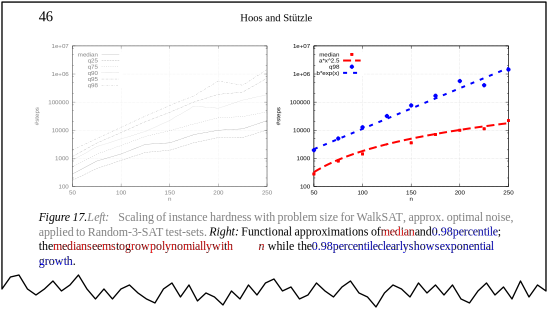
\includegraphics[width=\linewidth]{\sharedDir/graphics/papers/HS2000LSAFSAEEp46}\\%
{\small{(Taken from the paper \emph{\citetitle{HS2000LSAFSAEE}} by \citeauthor{HS2000LSAFSAEE}, coloring added manually\cite{HS2000LSAFSAEE}\tiny{, copyright Springer}.)%
}}}}}}{0.14}{0.14}%
%
\end{frame}%
%
%
%
\begin{frame}%
\frametitle{Geometric Mean}%
%
OK, arithmetic mean, median {\dots} but what about the geometric mean?%
%
\uncover<2->{%
\begin{definition*}[Geometric Mean]%
The geometric mean~\geoMeanb{A} is the $n$\textsuperscript{th} root of the product of $n$ \alert{positive} values.%
\uncover<3->{%
\begin{eqnarray}%
\geoMeanb{A} &=& \sqrt[n]{\prod_{i=0}^{n-1} \arrayIndex{a}{i}}\\\uncover<4->{%
\geoMeanb{A} &=& \exp{\left(\frac{1}{n} \sum_{i=0}^{n-1} \log{\arrayIndex{a}{i}} \right)}}%
\end{eqnarray}%
}%
\end{definition*}%
}%
\end{frame}%
%
\begin{frame}[t]%
\frametitle{Normalized Data}%
%
\begin{itemize}%
\item Often, our data is somehow \alert{normalized}.%
\only<-13>{\item<2-> Let's say we solve the problem instances $I_1$ to $I_3$ with the different algorithms $A_1$ to $A_3$.}%
\only<-14>{\item<3-> We measure the required runtimes as follows:}%
\only<-17>{\item<14-> The arithmetic mean\only<15->{\only<-15>{ and}\only<16->{,} the median\only<16->{, and the geometric mean}} values are the same.}%
\only<-18>{\item<17-> We can conclude that the three algorithms offer the same performance in average over these benchmark instances.}%
\only<-20>{\item<18-> But often the measured numbers \inQuotes{look messier} and are harder to compare at first glance.}%
\only<-21>{\item<19-> So often we want to normalize them by picking one algorithm as \inQuotes{standard} and dividing them by its measurements.}%
\only<-22>{\item<20-> Let's say \textcolor<21>{blue}{$A_1$} was a well-known heuristic, maybe we even took its results from a paper, and we want to use it as baseline for comparison and normalize our data by it.}%
\only<-26>{\item<22-> OK, so we get this table with normalized values, which allow us to make sense of the data at first glance.}%
\only<-29>{\item<23-> If we now compute the arithmetic mean\uncover<24->{, then \textcolor{displayGreen}{$A_1$ is best}\uncover<25->{ and \textcolor{red}{$A_3$ looks worst}.}}}%
\only<-29>{\item<26-> According to the median\uncover<27->{, \textcolor{displayGreen}{$A_3$ is best}\uncover<28->{ and \textcolor{red}{$A_2$ is worst!}}}}%
\only<-29>{\item<29-> Only the geometric mean still indicates that the algorithms perform the same\dots}%
\only<-32>{\item<30-> Hm.\uncover<31->{ OK, then let's normalize using the results of \textcolor{cyan}{$A_2$} instead.}}%
\only<-36>{\item<32-> OK, so we get this table with normalized values.}%
\only<-39>{\item<33-> If we now compute the arithmetic mean\uncover<34->{, then \textcolor{displayGreen}{$A_2$ is best}\uncover<35->{ and \textcolor{red}{$A_1$ looks worst}.}}}%
\only<-39>{\item<36-> According to the median\uncover<37->{, \textcolor{displayGreen}{$A_1$ is best}\uncover<38->{ and \textcolor{red}{$A_3$ is worst!}}}}%
\only<-40>{\item<39-> Only the geometric mean still indicates that the algorithms perform the same\dots}%
\item<40-> The geometric mean is the only meaningful average if we have \alert{normalized} data!\cite{FW1986HNTLWSTCWTSBR}%
\item<41-> And we very often have normalized data.%
\item<42-> For example, at least half of the papers on the \glsFull{optJSSP} normalize the result qualities they obtain on benchmark instances with the \glsFullpl{BKS}\only<-42>{\cite{W2019JRDAIOTJSSP}.}\uncover<43->{ and then compute the arithmetic mean\cite{W2019JRDAIOTJSSP}.}%
%
\end{itemize}%
%
\locate{4-39}{%
\resizebox{0.8\linewidth}{!}{%
\begin{tabular}{c@{\hspace{0.1\linewidth}}c}%
%
\begin{tabular}{rrrr}%
&\textcolor<21>{blue}{\textbf{$A_1$}}&\textbf{$A_2$}&\textbf{$A_3$}\\%
\textbf{$I_1$}&\textcolor<21-30>{blue}{\uncover<5->{10~s}}&\textcolor<31-39>{cyan}{\uncover<8->{20~s}}&\uncover<11->{40~s}\\%
\textbf{$I_2$}&\textcolor<21-30>{blue}{\uncover<6->{20~s}}&\textcolor<31-39>{cyan}{\uncover<9->{40~s}}&\uncover<12->{10~s}\\%
\textbf{$I_3$}&\textcolor<21-30>{blue}{\uncover<7->{40~s}}&\textcolor<31-39>{cyan}{\uncover<10->{10~s}}&\uncover<13->{20~s}\\%
\hline%
\uncover<14->{$\arithMean$:&23.33~s&23.33~s&23.33~s}\\%
\uncover<15->{$\median$:&20.00~s&20.00~s&20.00~s}\\%
\uncover<16->{$\geoMean$:&20.00~s&20.00~s&20.00~s}\\%
%
\end{tabular}
%
&%
%
\only<-31>{\uncover<22-30>{%
\begin{tabular}{rrrr}%
&\textcolor<22->{blue}{\textbf{$A_1$}}&\textbf{$A_2$}&\textbf{$A_3$}\\%
\textbf{$I_1$}&\textcolor<22->{blue}{1.00}&2.00&4.00\\%
\textbf{$I_2$}&\textcolor<22->{blue}{1.00}&2.00&0.50\\%
\textbf{$I_3$}&\textcolor<22->{blue}{1.00}&0.25&0.50\\%
\hline%
\uncover<23->{$\arithMean$:&\textcolor<24->{displayGreen}{1.00}&1.42&\textcolor<25->{red}{1.67}}\\%
\uncover<26->{$\median$:&1.00&\textcolor<28->{red}{2.00}&\textcolor<27->{displayGreen}{0.50}}\\%
\uncover<29->{$\geoMean$:&1.00&1.00&1.00}\\%
\end{tabular}%
}}%
%
\only<32->{\uncover<32->{%
\begin{tabular}{rrrr}%
&\textbf{$A_1$}&\textcolor{cyan}{\textbf{$A_2$}}&\textbf{$A_3$}\\%
\textbf{$I_1$}&0.50&\textcolor{cyan}{1.00}&2.00\\%
\textbf{$I_2$}&0.50&\textcolor{cyan}{1.00}&0.25\\%
\textbf{$I_3$}&4.00&\textcolor{cyan}{1.00}&2.00\\%
\hline%
\uncover<33->{$\arithMean$:&\textcolor<35->{red}{1.67}&\textcolor<34->{displayGreen}{1.00}&1.42}\\%
\uncover<36->{$\median$:&\textcolor<37->{displayGreen}{0.50}&1.00&\textcolor<38->{red}{2.00}}\\%
\uncover<39->{$\geoMean$:&1.00&1.00&1.00}\\%
\end{tabular}%
}}%
%
\end{tabular}%
}}{0.1}{0.5}%
%
\end{frame}%
%
\begin{frame}[t]%
\frametitle{Arithmetic Mean vs.\ Median vs.\ Geometric Mean}%
\begin{itemize}%
%
\item Most publications report arithmetic mean results, many report median results, almost none report geometric means.%
%
\item<2-> The median is more robust against outliers compared to the arithmetic mean\only<-2>{.}\uncover<3->{, however, in normal application scenarios, there are very few acceptable reasons for outliers.}%
\item<4-> We therefore want to know both the arithmetic mean and the median\only<4,10->{.}\only<-9>{\only<5->{:%
\begin{itemize}%
\item If the arithmetic mean is much worse than the median, then\uncover<6->{%
\begin{itemize}%
\item maybe we have a bug in our code that only sometimes has an impact\only<-6>{.}\uncover<7->{ or}%
\item<7-> our algorithm has a bad worst-case behavior (which is also good to know).%
\end{itemize}%
}%
%
\item<8-> If the median is much worse than the mean, then the mean is too optimistic, i.e., most of the time we should expect worse results.%
\end{itemize}}%
%
\item<9-> If there are outliers, the value of the arithmetic mean itself may be very different from any actually observed value, while the median is (almost always) similar to some actual measurements.%
}%
%
\item<11-> Often, our data is implicitly or explicitly normalized\only<-11>{.}\uncover<12->{, e.g.,%
\begin{itemize}%
\item if we divide result qualities by results of well-known heuristics or \glspl{BKS}\uncover<11->{ or}%
\item<13-> if we normalize the runtime using another algorithm as standard.%
\end{itemize}}%
\item<14-> Then, the arithmetic mean and median can be very misleading and the geometric mean must be computed.%
%
\item<15-> \alert{I think: On raw data, compute all three measures of average, and pay special attention to the one looking the worst.\uncover<16->{ On normalized data, compute the geometric mean\only<-16>{.}\uncover<17->{, but also consider the arithmetic mean and median \emph{if and only if they make \textbf{your} algorithm look worse}.}}}%
\end{itemize}%
%
\end{frame}%
%
\subsection{Measures of the Spread}%
%
\begin{frame}%
\frametitle{Measures of the Spread}%
\begin{itemize}%
\item The average gives us a good impression about the central value or location of a distribution.%
\item<2-> It does not tell us much about the range of the data.%
\item<3-> We do not know whether the data we have measured is very similar to the median or whether it may differ very much from the mean.%
\item<4-> An average alone is not very meaningful -- if we known nothing about the range of the data.%
\item<5-> We can therefore compute a measure of dispersion, i.e., a value that tells us whether the observations are stretched and spread far or squeezed tight around the center.%
\end{itemize}%
\end{frame}%
%
\begin{frame}%
\frametitle{Sample Variance}%
\begin{definition*}[Variance]%
The variance of a distribution is the expectation of the squared deviation of the underlying random variable from its expected value.%
\end{definition*}%
\uncover<2->{%
\begin{definition*}[Sample Variance]%
The variance~\sampleVarb{A} of a data sample~$A=(\arrayIndex{a}{0},\arrayIndex{a}{1}, \dots, \arrayIndex{a}{n-1})$ with $n$~observations can be estimated as:%
\begin{equation}%
\sampleVarb{A} = \frac{1}{n-1} \sum_{i=0}^{n-1} \left(\arrayIndex{a}{i} - \arithMeanb{A}\right)^2=\frac{1}{n-1}\left[ \left(\sum_{i=0}^{n-1}\arrayIndex{a}{i}^2\right) - \frac{1}{n}\left(\sum_{i=0}^{n-1}\arrayIndex{a}{i}\right)^2\right]%
\nonumber%
\end{equation}%
\end{definition*}%
}%
\end{frame}%
%
\begin{frame}%
\frametitle{Standard Deviation}%
\begin{definition*}[Sample Standard Deviation]%
\sloppy%
The standard deviation~\sampleStdDevb{A} of a data sample~$A=(\arrayIndex{a}{0},\arrayIndex{a}{1}, \dots, \arrayIndex{a}{n-1})$ with $n$~observations is the square root of the estimated variance~$\sampleVarb{A}$.%
\begin{equation}%
\sampleStdDevb{A} = \sqrt{\sampleVarb{A}}%
\nonumber%
\end{equation}%
\end{definition*}\fussy%
\end{frame}%
%
\begin{frame}%
\frametitle{Standard Deviation}%
\begin{itemize}%
\item Small standard deviations indicate that the observations tend to be similar to the mean.%
\item<2-> Large standard deviations indicate that they tend to be far from the mean.%
\item<3-> Small standard deviations in optimization results and runtime indicate that the algorithm is reliable.%
\item<4-> Large standard deviations indicate unreliable algorithms\only<-4>{.}\uncover<5->{, but may also offer a potential that could be exploited\only<-5>{.}\uncover<6->{: Given enough time, we can restart algorithms several times and expect to get different (and thus sometimes better) solutions.}}%
\end{itemize}%
\end{frame}%
%
\begin{frame}[t]%
\frametitle{Quantiles}%
\begin{definition*}[Sample Quantile]%
The $q$\nobreakdashes-quantiles are the cut points that divide a sorted data sample~$A=(\arrayIndex{a}{0},\arrayIndex{a}{1}, \dots, \arrayIndex{a}{n-1})$ where $\arrayIndex{a}{i-1}\leq \arrayIndex{a}{i} \; \forall i \in 1\dots (n-1)$ into $q$ equally-sized parts.%
\uncover<2->{ \sampleQuantile{k}{q}{A}~be the $k$\textsuperscript{th}~$q$\nobreakdashes-quantile, with $k\in 1\dots (q-1)$, i.e., there are $q-1$ of the $q$\nobreakdashes-quantiles.%
%
\begin{equation}%
\begin{array}{rcl}
h&=&(n-1)\frac{k}{q}\\
\sampleQuantile{k}{q}{A} &=& \left\{\begin{array}{ll}
\arrayIndex{a}{h}&\text{if~}h\text{~is integer}\\
\arrayIndex{a}{\lfloor h\rfloor}+\left(h-\lfloor h\rfloor\right)*\left(\arrayIndex{a}{\lfloor h\rfloor+1}-\arrayIndex{a}{\lfloor h\rfloor}\right)&\text{otherwise}
\end{array}\right.\end{array}\nonumber%
\end{equation}%
}%
\end{definition*}%
%
\uncover<3->{%
\begin{itemize}%
\item Quantiles are a generalized form of the median.%
\item<4-> The $\sampleQuantile{2}{1}{A}$ is the median of $A$%
\item<5-> 4-quantiles are called \emph{quartiles}.%
\item<6-> We often consider \emph{percentiles} or write things like \inQuotes{98\%~quantile} or \inQuotes{0.98~percentile} or \inQuotes{98\%~percentile} meaning~$\pgls{sampleQuantileMark}^{98}_{100}$.%
\end{itemize}%
}%
\end{frame}%
%
\begin{frame}%
\frametitle{Standard Deviation: Example}%
\begin{itemize}%
\item Two data samples $A$ and $B$ with $n_a=n_b=19$ values.%
\end{itemize}%
\uncover<2->{%
\begin{eqnarray}%
A &=& {\footnotesize{(1, 3, 4, 4, 4, 5, 6, 6, 6, 6, 7, 7, 9, 9, 9, 10, 11, 12, 14)}}\nonumber\\%
\only<-4>{\arithMeanb{A}&=&7\nonumber\\}%
B &=& {\footnotesize{(1, 3, 4, 4, 4, 5, 6, 6, 6, 6, 7, 7, 9, 9, 9, 10, 11, 12, \textcolor{red}{10'008})}}\nonumber%
\only<-4>{\\\arithMeanb{B}&=&533\nonumber}%
\uncover<3->{\\%
\sampleVarb{A} &=& \frac{1}{19-1} \sum_{i=1}^{19}\left(a_i-\arithMeanb{A}\right)^2 = \frac{198}{18}=11\nonumber\\%
\sampleVarb{B} &=& \frac{1}{19-1} \sum_{i=1}^{19}\left(b_i-\arithMeanb{B}\right)^2 = \frac{94'763'306}{18}\approx5'264'628\nonumber%
\uncover<4->{\\%
\sampleStdDevb{A}&=&\sqrt{\sampleVar{A}}=\sqrt{11}\approx{3.3}\nonumber\\%
\sampleStdDevb{B}&=&\sqrt{\sampleVar{B}}=\sqrt{\frac{94'763'306}{18}}\approx{2294}\nonumber%
}}%
\end{eqnarray}%
\uncover<5->{\vspace*{-1.1em}%
\begin{itemize}%
\item Being based on the arithmetic mean, the variance and standard deviation are heavily influenced by outliers -- with all pros and cons coming with that\dots%
\end{itemize}%
}}%
\end{frame}%
%
\begin{frame}%
\frametitle{Quantiles: Example}%
\begin{itemize}%
\item Two data samples $A$ and $B$ with $n_a=n_b=19$ values.%
\end{itemize}%
\uncover<2->{%
\begin{eqnarray}%
A &=& {\scalebox{0.8}{(1, 3, 4, 4, 4, 5, 6, 6, 6, 6, 7, 7, 9, 9, 9, 10, 11, 12, 14)}}\nonumber\\%
B &=& {\scalebox{0.8}{(1, 3, 4, 4, 4, 5, 6, 6, 6, 6, 7, 7, 9, 9, 9, 10, 11, 12, \textcolor{red}{10'008})}}\nonumber%
\uncover<3->{\\%
\sampleQuantile{1}{4}{A}&=&\sampleQuantile{1}{4}{B}=4.5\nonumber\\
\sampleQuantile{3}{4}{A}&=&\sampleQuantile{3}{4}{B}=9\nonumber%
}%
\end{eqnarray}%
\uncover<4->{%
\begin{itemize}%
\item Being generalizations of the median, the quantiles are little influenced by outliers -- with all pros and cons coming with that\dots%
\end{itemize}%
}}%
\end{frame}%
%
\begin{frame}[t]%
\frametitle{Further Example}%
\begin{itemize}%
\item The implicit assumption that $\arithMean\pm\sampleStdDev$ is a meaningful range is not always true!%
\item<4-> Such a shape is possible in optimization\only<4>{!}\uncover<5->{:%
\begin{itemize}%
\item The global optimum marks a lower bound for the possible objective values.%
\item<6-> A good algorithm often returns results which are close-to-optimal.%
\item<7-> There may be a long tail of few but significantly worse runs.
\item<8-> A statement such as \emph{\inQuotes{For this \gls{optTSP}~instance, our algorithm can find tours with a length of $100\pm120$~km.}} makes little sense\dots%
\end{itemize}%
}%
\end{itemize}%
\locateGraphic{1}{width=0.6\paperwidth}{\sharedDir/graphics/skew/skew_1}{0.2}{0.24}%
\locateGraphic{2}{width=0.6\paperwidth}{\sharedDir/graphics/skew/skew_2}{0.2}{0.24}%
\locateGraphic{3}{width=0.6\paperwidth}{\sharedDir/graphics/skew/skew_3}{0.2}{0.24}%
\locateGraphic{4-7}{width=0.45\paperwidth}{\sharedDir/graphics/skew/skew_3}{0.275}{0.44}%
\end{frame}%
%
%
\section{Statistical Comparisons}%
%
\begin{frame}\frametitle{Introduction}%%
%
\begin{itemize}%
%
\item We can now, e.g., perform 20~runs each with two different optimization algorithms on one problem instance and compute the medians of a performance indicator.%
%
\item<2-> Likely, they will be different.%
%
\item<3-> For one of the two algorithms, the results will be better.%
%
\item<4-> \alert{What does this mean?}%
%
\item<5-> It means that one of the two algorithms is better\only<-5>{.}\uncover<6->{\alert<6>{~with a certain probability}.}%
%
\item<7-> If we say \emph{\inQuotes{$A$ is better than $B$,}} we have a certain probability~$p$ to be wrong.%
%
\item<8-> \alert{The statement \emph{\inQuotes{$A$ is better than $B$}} makes only sense after we have decided about an upper bound~$\alpha$ for the acceptable error probability~$p$!}~(and if~$p<\alpha$, obviously)%
%
\end{itemize}%
%
\end{frame}%
%
\begin{frame}\frametitle{Statistical Tests}%
%
\begin{itemize}%
%
\item Compare two data samples $A=(a_1,a_2,\dots)$ and $B=(b_1,b_2,\dots)$ and%
%
\item<2-> get a result (e.g., \emph{\inQuotes{The median of $A$ is bigger than the median of $B$}}) \alert{together with} an error probability~$p$ that the conclusion is wrong.%
%
\item<3-> If~$p$ is less than a \alert{previously chosen} significance level (upper bound) \ensuremath{\alpha}, we can accept the conclusion.%
%
\item<4-> Otherwise, the observation is not significant\only<-4>{.}\uncover<5->{ and must be ignored.}%
%
\item<6-> But how can we arrive at such statements? How can we even estimate a probability to be wrong?%
%
\item<7-> \alert{Disclaimer: I am not a mathematician. What follows are simplified explanations of concepts.}%
%
\end{itemize}%
%
\end{frame}%
%

\begin{frame}[t]\frametitle{Example for Underlying Idea}%
%
\locateGraphic{2}{width=0.65\paperwidth}{\sharedDir/graphics/coin/coin_head_tails}{0.175}{0.28}%
\locateGraphic{5}{width=0.45\paperwidth}{\sharedDir/graphics/coin/coin_toss}{0.275}{0.4}%
%
\begin{itemize}%
\item<1-> Coin flip game: We flip a coin. If it is heads, I give you 1~RMB, if it is tails, you give me 1~RMB.%
\item<3-> We play 160~times.%
\item<4-> I win 128~times. You win 32~times.%
%
\item<6-> Did I cheat? Is my coin \inQuotes{fixed?} (i.e., is your chance to win $\neq0.5$)%
\item<7-> \alert<6>{Assumption: I cheat.} (alternative hypothesis $H_1$)%
\item<8-> It is impossible to compute my winning probability if I cheated\dots%
\item<9-> \alert<7>{Counter-Assumption: I did not cheat.} (null hypothesis $H_0$)%
%
\item<10-> How likely is it that I win \alert{at least} 128 times if I did \alert{not} cheat?%
\item<11-> (What we will do right now is called \emph{binomial test}.)%
\end{itemize}%
\end{frame}%
%
%
\begin{frame}[t]\frametitle{Example for Underlying Idea}%
\begin{itemize}%
\item<1-> How likely is it that I win \alert{at least} 128 times if I did not cheat?%
\item<2-> Then, the probabilities for heads and tails are $q=P(\texttt{head})=P(\texttt{tail})=0.5$.%
\item<3-> Flipping a coin $n$ times is a Bernoulli Process%
\item<4-> The probability $P(k|n)$ to flip $k\in 0..n$ times heads (or tails) is thus:%
\only<4->{%
\begin{equation}%
P(k|n)=\binom{n}{k} 0.5^{k} * (1-0.5)^{n-k} = \binom{n}{k} 0.5^{k} * 0.5^{n-k} = \binom{n}{k} \frac{1}{2^n}\nonumber%
\nonumber\end{equation}%
}%
\item<5-> For winning \alert{at least} $z=128$ times, we need to compute:%
\begin{eqnarray}%
P(k\geq z|n) &=& \sum_{i=z}^n P(i|n)%
\only<6>{=\sum_{i=128}^{160} P(i|160) = \sum_{i=128}^{160} \left[\binom{160}{i} \frac{1}{2^{160}}\right]}%
\only<7->{=\frac{1}{2^{160}} \sum_{i=128}^{160}\binom{160}{i}}\nonumber%
\only<8>{\\&=& \scalebox{0.82}{\ensuremath{\frac{1'538'590'628'148'134'280'316'221'828'039'113}{365'375'409'332'725'729'550'921'208'179'070'754'913'983'135'744}}}}%
\only<9->{\approx \ensuremath{\frac{1.539*10^{33}}{3.654*10^{47}}}}%
\only<10>{\\&\approx& \ensuremath{0.00000000000000421098571}}%
\only<11->{\\&\approx& \ensuremath{4.211\cdot10^{-15}}}%
\nonumber\end{eqnarray}%
\end{itemize}%
\end{frame}%
%
%
\begin{frame}\frametitle{Example for Underlying Idea}%
\begin{itemize}%
\item Question: How likely is it that I win at least 128 times if I did not cheat?%
\item<2-> If the coin was an ideal coin, the chance that I win at least 128 out of 160 times is about~$4\cdot10^{-15}$.%
\item<3-> If you claim that I cheat, your chance to be wrong is about~$4\cdot10^{-15}$.%
\item<4-> Thus, if we cannot accept a chance $p$ to be wrong higher than a significance level $\ensuremath{\alpha}=1\%$, we can still say:\bigskip\\%
{\strut\hfill\strut}\textbf{\alert{The observation is significant, I did likely cheat.}}{\strut\hfill\strut}%
%
\end{itemize}%
\end{frame}%
%
%
%
\begin{frame}[t]\frametitle{A More Specific Example for Tests}%
\begin{itemize}%
\item We want to compare two algorithms~$\mathcal{A}$ and~$\mathcal{B}$ on a given problem instance.
\item<2-> We have conducted a small experiment and measured objective values of their final results in a few runs in form of the two data sets~$A$ and~$B$, respectively:
\end{itemize}%
%
\uncover<2->{%
\begin{eqnarray}%
A &=& (2, 5, 6, 7, 9, 10)\nonumber\\%
B &=& (1, 3, 4, 8)\nonumber%
\end{eqnarray}%

\uncover<3->{%
\begin{itemize}%
\item From this, we can estimate the arithmetic means:
\end{itemize}%
%
\uncover<4->{%
\begin{eqnarray}%
\arithMeanb{A} &=& \frac{39}{6} = 6.5\nonumber\\%
\arithMeanb{B} &=& \frac{16}{4} = 4\nonumber%
\end{eqnarray}%
}}}%
%
\end{frame}%
%
%
\begin{frame}\frametitle{A More Specific Example}%
%%
\begin{eqnarray}%
\arithMeanb{A} &=& \frac{39}{6} = 6.5\nonumber\\%
\arithMeanb{B} &=& \frac{16}{4} = 4\nonumber%
\end{eqnarray}%
%
\begin{itemize}%
\item It looks like algorithm~$\mathcal{B}$ may produce the smaller objective values.
\item<2-> But is this assumption justified based on the data we have?
\item<3-> Is the difference between \arithMeanb{A} and \arithMeanb{B} significant at a threshold of $\alpha=2\%$?
\end{itemize}%
\end{frame}%
%
\begin{frame}\frametitle{A More Specific Example}%
%%
\begin{itemize}%
\item If~$\mathcal{B}$ is truly better than~$\mathcal{A}$, which is our hypothesis~$H_1$, then we cannot calculate anything.%
\item<2-> Let us therefore assume as null hypothesis~$H_0$ the observed difference did just happen by chance and, well, $\mathcal{A} \equiv \mathcal{B}$.
\item<3-> Then, this would mean that the data samples~$A$ and~$B$ stem from the \alert{same} algorithm (as $\mathcal{A} \equiv \mathcal{B}$).
\item<4-> The division into the two sets would only be artificial, an artifact of our experimental design.
\item<5-> Instead of having two data samples, we only have one, namely the union set~$O$ with~10 elements:
\end{itemize}%%
%
\uncover<6->{%
\begin{equation}%
O = A \cup B = (1, 2, 3, 4, 5, 6, 7, 8, 9, 10)%
\nonumber\end{equation}%
}%
%
\end{frame}%
%
%
\begin{frame}[t]\frametitle{A More Specific Example}%
%
\only<-5,8->{%
\addtocounter{equation}{-1}%
\begin{equation}%
O = A \cup B = (1, 2, 3, 4, 5, 6, 7, 8, 9, 10)%
\nonumber\end{equation}%
%
\begin{itemize}%
\item Any division $C$ into two sets with $4$ and $6$ elements has the same probability%
\item<2-> $|O|=10$%
\item<3-> There are ${10 \choose 4}={210}$ different ways to draw $4$ (or $6$) elements from $O$%
\item<4-> If $H_0$ holds, all have the same probability%
%
\only<5-7>{\item<5-7> Let's use a \python\cite{programmingWithPython} program to test the combinations}%
%
\item<8-> There are~27 such combinations with a mean of \alert<8>{less or equal~4}.%
%
\item<9-> The probability~$p$ to observe a situation at least as extreme as~$A$ and~$B$ under~$H_0$ is thus:%
\end{itemize}%
\uncover<10->{%
\begin{equation}%
p=\frac{\textnormal{\#cases~$C$}:\arithMeanb{C}\leq \arithMeanb{B}}{\textnormal{\#all cases}}=\frac{{27}}{{210}}=\frac{9}{70}\approx {0.1286}%
\nonumber\end{equation}%
}%
}%
%
\locateListingBox{6-7}{%
\lstinputlisting[style=python_style]{code/enumerate.py}%
}{0.1}{0.16}{0.8}{0.8}%
\gitExec{exec:enumerate}{}{}{python3 code/enumerate.py}%
%
\locateListingBox{7}{%
\lstinputlisting[style=text_style]{\gitFile{exec:enumerate}}
}{0.1}{0.775}{0.8}{0.4}%
%
\end{frame}
%
%
\begin{frame}[t]\frametitle{A More Specific Example}%
\begin{itemize}%
%
\item Extreme cases into the other direction are the same, because if $\arithMeanb{B}\leq 4$ then $\arithMeanb{A}\geq 6.5$ for any division $A\cup B=O$ and vice versa\only<-1>{.}\uncover<2->{:}%
\begin{footnotesize}%
\begin{eqnarray}
\only<1-5>{O &=& A \cup B = (1, 2, 3, 4, 5, 6, 7, 8, 9, 10)}\nonumber%
\only<2->{\only<1-5>{\\}%
\only<2-6>{\sum_{\forall o\in O} o &=& \sum_{o=1}^{10}o = \frac{10 (10+1)}{2} = 55}\nonumber%
\only<3->{\only<2-6>{\\}%
\arithMeanb{B} =\left(\frac{1}{4}\sum_{\forall b\in B}b\right) \leq 4 &\Longrightarrow& \left(\sum_{\forall b\in B}b\right) \leq 4*4 \leq 16\nonumber%
\only<4->{\\%
O=A\cup B&\Longrightarrow&\sum_{\forall a\in A}a = \left(\sum_{\forall o\in O}o\right)-\left(\sum_{\forall b\in B}b\right)\nonumber%
\only<5->{\\%
\sum_{\forall b\in B}b \leq 16 &\Longrightarrow& \left(\sum_{\forall a\in A}a \right) \geq 55-16\geq 39\nonumber%
\only<6->{\\%
\arithMeanb{A} &=& \frac{1}{6}\left(\sum_{\forall a\in A}a \right)\nonumber%
\only<7->{\\%
\arithMeanb{B} \leq 4 &\Rightarrow& \arithMeanb{A} \geq \frac{39}{6} \geq 6.5\nonumber%
}}}}}}%
\nonumber\end{eqnarray}%
\end{footnotesize}%
%
\item<8-> So -- of course -- we could have also done the test the other way around with the same result!%
%
\end{itemize}%
\end{frame}%
%
\begin{frame}[t]\frametitle{A More Specific Example}%
%
\begin{itemize}%
\item The probability~$p$ to observe a constallation at least as extreme as~$A$ or~$B$ under~$H_0$ is thus:%
\end{itemize}%
\addtocounter{equation}{-1}%
\begin{equation}%
p=\frac{\textnormal{\#cases~$C$}:\arithMeanb{C}\leq \arithMeanb{B}}{\textnormal{\#all cases}}=\frac{{27}}{{210}}=\frac{9}{70}\approx {0.1286}%
\nonumber\end{equation}%
%
\begin{itemize}%
\item<2-> If we claim that~$A$ and~$B$ are from distributions with means as different as observed\dots%
\item<3-> {\dots}we are wrong with probability $p\approx 0.13$
\item<4-> At a significance level of $\ensuremath{\alpha}=2\%$, the \alert{means} of~$A$ and~$B$ are not significantly different! ($2\%<0.13$)%
\item<5-> Actually: This here is an example for an \emph{Randomization Test}\cite{BLB2008VMIDBS,E1995RT}.%
\item<6-> \alert<6>{The method here is only feasible for small sample sets, real tests are more sophisticated}%
\end{itemize}%
%
\end{frame}%
%%
%
\begin{frame}[t]\frametitle{Statistical Tests: Types}%
%
\begin{itemize}%
%
\item<1-> Statistical tests are more elegant mathematical approaches than the example shown before.\uncover<2->{ In order to work, they have preconditions, they make certain assumptions.}%
\item<3-> There are two types of tests:%
%
\begin{enumerate}%
\item<4-> Parametric Tests%
%
%
\only<5-10>{%
\begin{itemize}%
\item Assume that the data samples follow a certain distribution%
\item<6-> Examples\cite{B2001MVORSNPM}: $t$-test (assumes normal distribution)%
\item<7-> The distribution of the data we measure is unknown\dots%
\item<8-> {\dots}and usually not normal nor symmetric (see the further quantiles/stddev plot example).%
\item<9-> The condition for using such tests often cannot be met (known distribution)%
\item<10-> \alert{Parametric tests should usually not be used here!}%
\end{itemize}%
}%
%
%
\item<11-> Non-Parametric Tests%%
\only<12->{%
\begin{itemize}%
\item Make few assumption about the distribution from which the data was sampled.%
\item<13-> Examples\cite{W2009GOATAA}: %
the \mbox{Wilcoxon rank sum test} with continuity correction (also called \mbox{Mann-Whitney U test\cite{B1972CCSURS,SC1988NSFTBS,HW1973NSM,MW1947OATOWOOTRVISLTTO}}), %
\mbox{Fisher's Exact Test\cite{F1922OTIOCFCTATCOP}}, %
the \mbox{Sign Test\cite{G2003SFNEIDSDWIWMEST,SC1988NSFTBS}}, %
the \mbox{Randomization Test\cite{BLB2008VMIDBS,E1995RT}}, and %
\mbox{Wilcoxon's Signed Rank Test\cite{W1945ICBRM}}.%
\item<14-> These tests are more \alert{robust} (less assumptions)%
\item<15-> \alert<15>{This usually is the kind of test we want to use.}%
\item<16-> They work similar to the previous test example, but with larger sample sizes%
\item<17-> \alert{Often, the most suitable test is the Mann-Whitney U test.}
\end{itemize}%
}%
%
\end{enumerate}%
\end{itemize}%
%
\end{frame}%
%
%
\begin{frame}\frametitle{A fair warning}%
\begin{itemize}%
\item There are many algorithms and even more configuration parameters.%
\item<2-> All kinds of algorithm modules and parameters have some kind of impact on the performance.%
\item<3-> If I have two different algorithms $\mathcal{A}$ and $\mathcal{B}$, logic dictates that their performance is also different.%
\item<4-> But is this difference usually significant?%
\item<5-> From the viewpoint of statistics: Probably \alert<5>{yes}.%
\item<6-> If I just conduct enough runs, maybe thousands, or millions, than even a difference of 0.001\% in performance will pass a test as \alert<6>{significant}.%
\item<7-> To be \alert{practically significant}, the measured difference of results should be \alert{large enough} and statistically significant already with few runs, say, 11 or 21, not just with $\geq100$ runs.%
\end{itemize}%
\end{frame}%
%
\begin{frame}[t]\frametitle{Compare $N\geq 2$ Algorithms}%
%
\only<-4,6-7>{%
\begin{itemize}%
\item For comparing $N\geq 2$ algorithms, we can compare any two algorithms with each other%
\only<2->{%
\item<2-> $N$ Algorithms $\Rightarrow$ $k=N(N-1)/2$ statistical tests\only<-4>{ (e.g., Mann-Whitney U)}%
\only<3->{%
\item<3-> $k$ tests and each with error proability \ensuremath{\alpha}\only<4->{ $\Longrightarrow$ %
total probability $E$ to make at least one error $E=1-((1-\ensuremath{\alpha})^k)$%
\item<6-> Correction needed\uncover<7->{: Bonferroni correction\cite{D1961MCAM}\uncover<6->{:~Use $\ensuremath{\alpha}'=\ensuremath{\alpha}/k$ as significance level instead of $\ensuremath{\alpha}$, then the overall probability $E$ to make an error will remain $E\leq\ensuremath{\alpha}$.}}%
}}}%
\end{itemize}%
}%
\locateGraphic{5}{width=0.9\paperwidth}{\sharedDir/graphics/errorProb/multicomp_bonferroni_error}{0.05}{0.22}%
\locateGraphic{8}{width=0.9\paperwidth}{\sharedDir/graphics/errorProb/multicomp_bonferroni_corrected}{0.05}{0.22}%
\end{frame}%
%
%
\section{Testing is Not Enough}%
%
%
\begin{frame}\frametitle{The question of termination}%
%
\only<-2,4-6,11->{%
\begin{itemize}%
%
\item Literature usually reports tuples \inQuotes{$(\textnormal{instance}, \textnormal{result}, \textnormal{runtime})$}%
%
\item<2-> \only<4->{\textcolor<-4>{red}{Problem}: }Papers often use different termination criteria%%
%
\item<5-> Anytime Algorithms\cite{BD1989STDPP2}\uncover<6->{: Always have approximate solution, refine it iteratively}%
%
\item<11-> \textcolor<-11>{red}{One measure point per run or instance does not tell the whole story!}%
%
\item<12-> Using statistical tests cannot solve this issue (still: at one point in time).%
%
\item<13-> We should have the \inQuotes{whole performance curves!}\uncover<14->{ {\dots} ideally mean or median curves over several runs!}%
%
\end{itemize}%
}%
%
\locateGraphic{3}{width=0.7\paperwidth}{\sharedDir/graphics/termination/points}{0.15}{0.24}%
\locateGraphic{7}{width=0.7\paperwidth}{\sharedDir/graphics/termination/points}{0.15}{0.24}%
\locateGraphic{8}{width=0.7\paperwidth}{\sharedDir/graphics/termination/lines}{0.15}{0.24}%
\locateGraphic{9}{width=0.7\paperwidth}{\sharedDir/graphics/performance_dimensions/performance_dimensions}{0.15}{0.24}%
\locateGraphic{10}{width=0.7\paperwidth}{\sharedDir/graphics/performance_cuts/performance_cuts}{0.15}{0.24}%
%
\end{frame}%
%
\section{Other Stuff}%
%
\begin{frame}\frametitle{New Algorithms and Problems}%
\begin{itemize}%
\item There are many papers that introduce two things at the same time: a new optimization problem and a new algorithm.\uncover<2->{ \alert{I think this is not a good idea.}}%
\item<3-> If we introduce a new optimization algorithm, we should test it on well-known, well-established benchmark problems.\uncover<4->{ For such problems, results from other well-known and well-established algorithms exist -- so we can compare our algorithm to them and investigate its performance objectively.}%
\item<5-> If we introduce a new optimization problem, we should apply well-known and well-established algorithms to it.\uncover<6->{ This way we get proper baseline results and can understand whether the problem is hard for the state-of-the-art and/or how far this state-of-the-art allows us to go.}%
\item<7-> If we have two \inQuotes{moving parts} at the same time, it is hard to understand whether an algorithm is good and whether a problem is hard.%
\item<8-> If you have an own new algorithm on a new problem and use other algorithms for comparision, you might be tempted to just use the most basic configurations of these algorithms.\uncover<9->{ Then your algorithm might look good, while it actually is not.}%
\item<10> \alert{Know the standard benchmark instances for your field!}%
\end{itemize}%
\end{frame}%
%
\begin{frame}\frametitle{Reproducibility}%
\begin{itemize}%
\item Your experiments should be well-documented and reproducible.%
\item<2-> In the ideal case, someone else can run your code and get the same results.%
\item<3-> For this purpose, you should make your code available, e.g., put it on \github\ or zenodo.org.%
\item<4-> If your experiments are time-consuming, also make sure to properly store all your results in human- and machine-readable form, ideally in a \glsFull{CSV} format.%
\item<5-> You should make an archive such that a)~I can directly run the same experiments that you did and b)~also have all the data and tools to create the same statistics and figures.%
\item<6-> \alert{But what if someone finds an error in work?}%
\item<7-> That is OK.%
\item<8-> Better they find it in your \alert{code} that you voluntarily provided than after going through significant re-implementation effort\dots%
\end{itemize}%
\end{frame}%
%
\begin{frame}[t]\frametitle{Cheating}%
\centering%
\alert{What are typical bad / cheating behavior in research on optimization?}\uncover<2->{%
\medskip%
\begin{itemize}%
\item Cherry-Picking\only<3-10>{:%
\begin{itemize}%
\item On a benchmark instance, many runs are conducted with different random seeds.\uncover<4->{ %
But only the 10 with the best results are reported.\uncover<5->{ %
This can be prevented by generating the sequence of random seeds with a deterministic algorithm and reporting both\cite{WW2023RSDEWASSAA}.}}%
\item<6-> Only the benchmark instances where the algorithm performs well are chosen.\uncover<7->{ %
Be wary of statements such as \inQuotes{We now present the results of our algorithm on 10 of the \gls{TSPLib} instances.} (\gls{TSPLib} has more than 100\dots)}%
\item<8-> Weak algorithms are chosen for comparison.\uncover<9->{ %
Comparison must always be done with the state-of-the-art on the specific problem at hand.\uncover<10->{ %
Be wary of statements such as \inQuotes{We compare our algorithm with the standard Genetic Algorithm.} (because the SGA is usually not the state-of-the-art)}}%
\end{itemize}}%
\item<11-> Sometimes, results may be straight up fabricated.\only<12>{ %
Algorithm must be clearly specified and ideally the source code is available to prevent this.}%
\item<13-> Misleading statistics are reported\only<13>{ (see our discussion on normalization).}%
\item<14-> Uneven configuration effort\only<15->{.}\only<14>{: Much effort is spent on configuring the own algorithm, the algorithms used for comparison are used with bad settings.}%
\item<15-> Incomparable results are reported\only<15>{ (see our discussion on why testing is not enough)}.%
\item<16-> Misleading significance in test results (high~$\alpha$, many runs, no corrections).%
\end{itemize}}%
\medskip%
\uncover<17->{\alert{Reproducibility prevents cheating and misunderstandings!}}%
\end{frame}%
%
\section{Summary}%
%
\begin{frame}\frametitle{Summary}%
\begin{itemize}%
\item The optimization algorithms we consider in this lecture are \alert<1>{randomized}.%
%
\item<2-> Comparing them must be done in a \alert<2>{statistical way} using data from \alert<2>{multiple runs}%
%%
\item<3-> Two views on performance\uncover<4->{:%
\begin{enumerate}%
\item best result after fixed number of \glspl{objFE}/runtime%
\item<5-> number of \glspl{objFE}/runtime needed to get certain result%
\end{enumerate}%
}%
%
%
\item<6-> For every single algorithm/configuration, compute\uncover<7->{:%
\begin{enumerate}%
\item arithmetic and geometric mean and median of key performance indicators%
\item<8-> quartiles or top/bottom 1\% quantile to get a feeling for the usual range of values%
\item<9-> don't trust just arithmetic mean or standard deviation alone%
\item<10-> geometric mean if the data is normalized%
\end{enumerate}%
}%
%
\item<11-> Use non-parametric statistical tests with corrections for multiple comparisons.%
%
\item<12-> Do not only collect one data sample per run, try to plot progress curves.%
%
\item<13-> Use well-known benchmarks, provide your source code!%
%
\end{itemize}%
\end{frame}%
%
\section{Advertisement}%
%
\begin{frame}[t]%
\frametitle{Programming with Python}%
We have a freely available course book on \citetitle{programmingWithPython} at \citeurl{programmingWithPython}, with focus on practical software development using the \python\ ecosystem of tools\cite{programmingWithPython}.%
%
\locateGraphic{}{width=0.63\paperwidth}{\sharedDir/graphics/advertisement/snippets/programmingWithPythonSnippet}{0.025}{0.3}%
\locateGraphic{}{width=0.27\paperwidth}{\sharedDir/graphics/advertisement/urlQr/programmingWithPythonCourseUrl}{0.675}{0.4}%
%
\end{frame}%
%
\begin{frame}[t]%
\frametitle{Databases}%
We have a freely available course book on \citetitle{databases} at \citeurl{databases}, with actual practical examples using a real \dbms\cite{databases}.%
%
\locateGraphic{}{width=0.63\paperwidth}{\sharedDir/graphics/advertisement/snippets/databasesSnippet}{0.025}{0.3}%
\locateGraphic{}{width=0.27\paperwidth}{\sharedDir/graphics/advertisement/urlQr/databasesCourseUrl}{0.675}{0.4}%
%
\end{frame}%
%
%
\endPresentation%
\end{document}%%
\endinput%
%
